\begin{frame}{introduction}{artificial intelligence}
    \vspace{-3mm}
    \begin{columns}
    \column{.65\linewidth}
        \begin{itemize}
            \item \textbf{artificial intelligence}
                \begin{itemize}
                    \item unclear definition: everything that is perceived to act intelligently
                    \item   changes over time
                \end{itemize}
            \bigskip
            \item \textbf{machine learning}
                \begin{itemize}
                    \item   data-driven: algorithm is more agnostic to task and is parametrized through training with data
                \end{itemize}
            \bigskip
            \item   \textbf{deep learning}
                \begin{itemize}
                    \item deep neural networks are 'the algorithm'
                \end{itemize}
        \end{itemize}
    \column{.35\linewidth}
        \begin{figure}%
            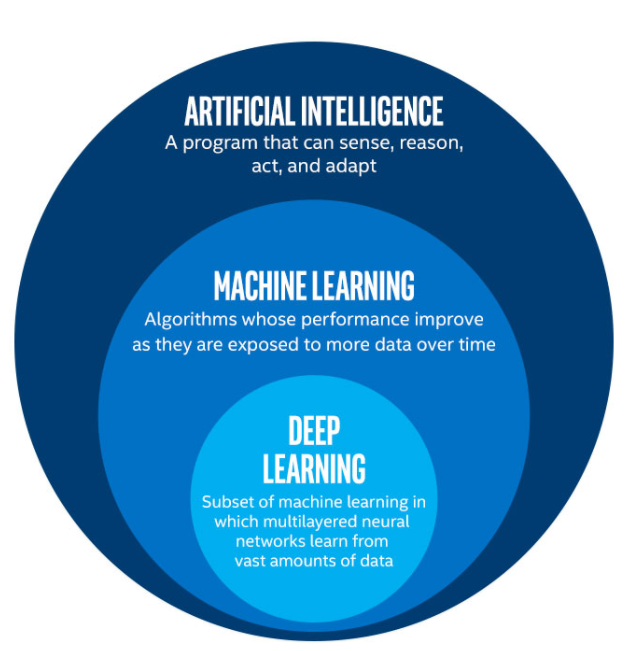
\includegraphics[width=\columnwidth]{ai-ml-dl}%
        \end{figure}
    \end{columns}
\end{frame}

\begin{frame}{machine learning}{importance of data}
    \vspace{-5mm}
    \begin{textblock*}{100mm}(0cm,1.5cm)
        
\includegraphics[scale=.1]{machinelearning}
    \end{textblock*}           
    
    \begin{columns}
    \column{.6\linewidth}
    \begin{itemize}
 
        \item<1->   \textbf{machine learning}: generic algorithm mapping an input to an output
            \begin{itemize}
                \item<2->   mapping function is learned from patterns and characteristics \textbf{from data}
                \item<2->[$\Rightarrow$]   model \textbf{success largely depends on training data}
                
            \end{itemize}
        \bigskip
        \item<3->   \textbf{technical challenges} concerning data
            \begin{itemize}
                \item   \textit{imbalance \& bias} (data distribution is skewed, biased)
                \item   \textit{diversity \& representativeness} (data does not reflect target distribution)
                \item   \textit{subjectivity} of annotations
                \item   \textit{noisiness} (bad quality, bad annotations, unrelated data points, ...)
                \item   amount
            \end{itemize}
    \end{itemize}
    \column{.4\linewidth}
        \begin{figure}
            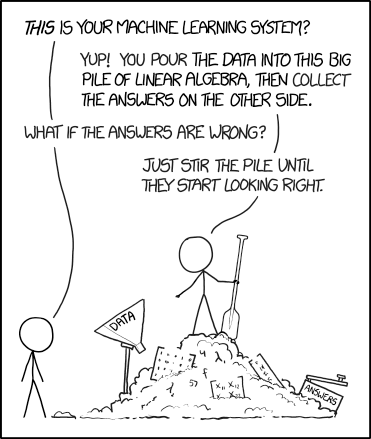
\includegraphics[scale=.4]{machine_learning}
        \end{figure}
    \end{columns}
    \addreference{\href{https://imgs.xkcd.com/comics/machine\_learning.png}{https://imgs.xkcd.com/comics/machine\_learning.png}}
\end{frame}

        \begin{frame}{introduction}{machine learning categorization based on output types}
            \begin{itemize}
                \item \textbf{classification}:\\ input data is categorized into pre-determined output categories (e.g., music genres)
                \smallskip
                \item \textbf{clustering}:\\ input data is grouped into prevalent clusters (no pre-determined categories)
                \smallskip
                \item \textbf{regression}:\\ predict a numerical value based on an input (e.g., estimate how danceable a piece of music is)
                \smallskip
                \item \textbf{generation}:\\ input is control data, output is target data (e.g., a composition)
            \end{itemize}
        \end{frame}
        
        %\begin{frame}{introduction}{audio classification --- traditional}
            %\vspace{-3mm}\begin{textblock*}{100mm}(.5cm,2.5cm)
                %\includegraphics[scale=.2]{waveform}
            %\end{textblock*}
            %\begin{figure}
                %\centering
								%\begin{footnotesize}
									%\begin{picture}(96,26)
										%\setcounter{iXOffset}{0}
										%\setcounter{iYOffset}{5}
										%\setcounter{iXBlockSize}{28}
										%\setcounter{iYBlockSize}{16}
										%\setcounter{iYBlockSizeDiv2}{8}
										%\setcounter{iDistance}{8}
%
										%\addtocounter{iYOffset}{\value{iYBlockSizeDiv2}}
										%\addtocounter{iYOffset}{-2}
%
										%%\addtocounter{iXOffset}{-1}
										%\put(\value{iXOffset}, \value{iYOffset})
											%{\text{{\shortstack[c]{audio\\ signal}}}}
										%\addtocounter{iXOffset}{1}
%
										%\addtocounter{iYOffset}{2}
										%\addtocounter{iXOffset}{\value{iDistance}}
%
										%\put(\value{iXOffset}, \value{iYOffset})
											%{\vector(1,0){\value{iDistance}}}
%
										%\addtocounter{iXOffset}{\value{iDistance}}
										%\addtocounter{iYOffset}{-\value{iYBlockSizeDiv2}}
										%
										%\put(\value{iXOffset}, \value{iYOffset})
											%{\framebox(\value{iXBlockSize}, \value{iYBlockSize}) {\shortstack[c]{feature extraction}}}
%
										%\addtocounter{iXOffset}{\value{iXBlockSize}}
										%\addtocounter{iYOffset}{\value{iYBlockSizeDiv2}}
%
										%\put(\value{iXOffset}, \value{iYOffset})
											%{\vector(1,0){\value{iDistance}}}
%
										%\addtocounter{iXOffset}{\value{iDistance}}
										%\addtocounter{iYOffset}{-\value{iYBlockSizeDiv2}}
%
										%\put(\value{iXOffset}, \value{iYOffset})
											%{\framebox(\value{iXBlockSize}, \value{iYBlockSize}) {\shortstack[c]{classification,\\ inference}}}
%
										%\addtocounter{iXOffset}{\value{iXBlockSize}}
										%\addtocounter{iYOffset}{\value{iYBlockSizeDiv2}}
%
										%\put(\value{iXOffset}, \value{iYOffset})
											%{\vector(1,0){\value{iDistance}}}
%
										%\addtocounter{iXOffset}{\value{iDistance}}
										%\addtocounter{iYOffset}{-2}
%
										%\addtocounter{iXOffset}{1}
										%\put(\value{iXOffset}, \value{iYOffset})
											%{\text{{\shortstack[c]{class\\ labels}}}}
										%
									%\end{picture}
								%\end{footnotesize}
            %\end{figure}
            %
            %\vspace{-5mm}
            %\begin{columns}
                %\column{.5\textwidth}
                    %\begin{itemize}
                        %\item<2->[]	\textbf{feature} representation
                                %\begin{itemize}
                                    %\item 	compact and non-redundant
                                    %\item	task-relevant
                                    %\item   easy to analyze
                                    %\item   e.g., MFCCs etc.
                                %\end{itemize}
                    %\end{itemize}
                %\column{.5\textwidth}
                    %\begin{itemize}
                        %\item<3->[]	\textbf{classification}
                                %\begin{itemize}
                                    %\item	map or convert feature to comprehensible domain
                                    %\item   e.g., Support Vector Machines etc.
                                %\end{itemize}
                    %\end{itemize}
            %\end{columns}
            %\phantom{\footfullcite{burred_hierarchical_2004}}
        %\end{frame}
        %
        %\begin{frame}{introduction}{neural network based approaches}
            %\vspace{-3mm}
            %\begin{itemize}
                %\item   no custom-designed features anymore
                %\item   learn features from basic inputs (like spectrograms)
            %\end{itemize}
            %\begin{figure}%
                %\includegraphics[width=\columnwidth]{audio_classification}%
            %\end{figure}
            %\addreference{Fig.: \href{https://towardsdatascience.com/audio-deep-learning-made-simple-sound-classification-step-by-step-cebc936bbe5}{towardsdatascience.com}}
            %\pause
            %\begin{itemize}
                %\item   less required expert-knowledge, more complex systems
                %\item   less expert-tweaking, more rigorous experimental requirement
                %\item   much \textcolor{gtgold}{\textbf{higher data requirements}}
            %\end{itemize}
            %
        %\end{frame}
